%
% Adaptation of the Thesis Template bei Philip Döbler shared under CC-BY 3.0
% Ergänzungen von:
% Till Tantau (teilweise entfernt)
% André Calero Valdez
% Tim Schrills


\documentclass[
    paper = a4,
    fontsize = 12pt,
    headinclude = true,
    % start chapters on the right side
    open = right,
    % Use twosided layout? Every chapter starts on the right side, therefore sometimes blank pages are added between chapters.
    twoside = false,
    BCOR = 10mm,
    % add lists and bibliography to table of contents
    toc = listofnumbered,
    toc = bibnumbered,
    % enumerate chapters as x.y instead of x.y.
    numbers = noendperiod
]{scrreprt}

% use some additional package, add your own below if required
\usepackage[utf8]{inputenc}
\usepackage[T1]{fontenc}
% package for code listings
\usepackage{listings}
% package providing colors (e.g. for syntax highlighting in listings)
\usepackage{xcolor}
% package for german language, change to english if required
\usepackage[ngerman]{babel}
\usepackage[german=quotes]{csquotes}
\usepackage{xpatch}
\usepackage{hyphenat}
% package to set the line spacing
\usepackage{setspace}
% package for hyperlinks (e.g., in the table of contents) and set links to same style as text
\usepackage[hidelinks]{hyperref}
% package to create acronyms
\usepackage[acronym]{glossaries}
% package for pseudocode
\usepackage[german, algochapter, linesnumbered]{algorithm2e}
% package to create diagrams
\usepackage{tikz}
\usepackage{booktabs}
\usepackage{float} % in der Präambel
\usepackage{lmodern}
\usepackage{array}
\usetikzlibrary{positioning}
\usetikzlibrary{shapes.geometric, arrows}
\tikzset{font={\fontsize{10pt}{12}\selectfont}}

%%% additions by ACV
% Citations using APA style with biblatex
\usepackage[style=verbose,backend=biber,backref=true,maxbibnames=20]{biblatex}
% Biblatex allows multiple bib-files
\addbibresource{bibliography/references.bib}
\addbibresource{bibliography/websources.bib}
\addbibresource{bibliography/normen.bib}

% Tables using APA Style
\usepackage{booktabs}

% use microkerning for improved typesetting
\usepackage{microtype}

% include acronyms
% add acronyms below
\newacronym{nic}{NIC}{Network Interface Controller}


% avoid bold caption for algorithms to be consistent with other captions
\SetAlCapSty{}
\SetNlSty{footnotesize}{}{}

% definitions for syntax highlighting in listings environment
% define custom colors for syntax highlighting in code listings
\definecolor{lst_comments}{rgb}{0, 0.75, 0}
\definecolor{lst_linenumbers}{rgb}{0.2, 0.2, 0.2}
\definecolor{lst_keywords}{rgb}{0, 0, 0.75}
\definecolor{lst_strings}{rgb}{0.75, 0, 0}
\definecolor{lst_background}{rgb}{0.97, 0.97, 0.97}

% define style for listings
\lstdefinestyle{msqc_style}{
    backgroundcolor=\color{lst_background},   
    commentstyle=\color{lst_comments},
    keywordstyle=\color{lst_keywords},
    stringstyle=\color{lst_strings},
    % style of the line numbers on the left side
    numberstyle=\tiny\color{lst_linenumbers},
    % use monospace font for code and set size to the size of footnotes
    basicstyle=\footnotesize,
    xleftmargin=2em,
    % break long lines, if this happens it might be better to manually add a line break at an appropriate place
    breaklines = true,
    % place caption below the listing
    captionpos = b,
    % don't drop spaces to fix alignment and always convert tabs to spaces
    keepspaces = true,
    % place line numbers on the left side
    numbers = left,
    % distance between line numbers and listing
    numbersep = 7pt,
    % don't show special characters for spaces
    showspaces = false,
    % don't show special characters for spaces in strings
    showstringspaces = false,
    % don't show special characters for tabs
    showtabs = false,
    % set size of tab to 4 spaces
    tabsize = 4
}
% set style for the document
\lstset{style=msqc_style}

% set line spacing to 1.5
\onehalfspacing

\begin{document}
    % use roman numbering for preamble
    \pagenumbering{Roman}
    % add title page and abstract
    \begin{titlepage}
    \begin{center}
        %% TODO: find hires figure.
        
\includegraphics{figures/HFT-Logo.jpg}\\
        \normalsize
        \sffamily
        %{\color{gray}Direktor:in Prof. Dr. rer. nat. Nicole Jochems\\}
        
        \vspace{0.5cm} 
        
        \Huge
        \textbf{Betreutes Praktisches Studienprojekt}
        \vfill
        
        \normalsize
        % change accordingly for Master Thesis
        \textbf{Praktikumsbericht} \\
        \vspace{0.4cm}
        
        im Rahmen des Studiengangs\\
        \textbf{Wirtschaftsinformatik}\\
        der Hochschule für Technik Stuttgart\\

        
        \vspace{0.8cm}
        vorgelegt von: \\
        \large
        \textbf{Julian Raubald}\\ 
        (Matrikelnummer 1003812)\\
        
        \normalsize
        \vspace{0.8cm}
        Praktikumsbetrieb:\\ 
        \large
        %\textbf{iteratec GmbH}\\
        
\includegraphics[width=0.5\textwidth]{figures/iteratec-Logo.png}\\
        \vspace{0.3cm}
        \normalsize
        Betreut durch:\> \\ 
        \large
        \textbf{Prof. Dr. Stefan Knauth} \\
        \normalsize
        \vspace{0.5cm}
        Stuttgart, Tag. Februar. 2024\\
    \end{center}
\end{titlepage}
    
    % print table of contents
    \tableofcontents
    
    % use arabic numbering for main part
    \cleardoublepage\pagenumbering{arabic}

    % Deutsche Paragrapheinzüge auf 0 und Parskip auf 10 pt
    % Für englische Text auskommentieren
    \setlength{\parindent}{0pt}
    \setlength{\parskip}{10pt}
    
    % create a tex file for each chapter and include it below

    %%%%%%%%%%%%%%%%%%%%%%%%%%%%%%%%
    %%%%%%%%%%%%%%%%%%%%%%%%%%%%%%%% 
    % Inhalt der Arbeit
    \chapter{Einleitung}
In diesem Bericht schildere ich die Aufgaben und Projekte, welche ich in meinem Praxissemester im Wintersemester 23/24
bei dem Unternehmen iteratec GmbH durchgeführt und begleitet habe. Dabei gehe ich auf die eingesetzten Technologien ein
und teile meine gesammelten Erfahrungen und ordne diese inhaltlich im Rahmen meines Studiums der Wirtschaftsinformatik
ein.

\section{Unternehmen iteratec GmbH}

Iteratec ist ein Unternehmen, das sich auf digitale Produktinnovation, Software- und Architekturentwicklung sowie
digitale Infrastrukturen spezialisiert hat. Als Partner für die digitale Transformation unterstützt es Unternehmen und
öffentliche Organisationen bei der Digitalisierung ihrer Prozesse, Produkte und Dienstleistungen. Dies umfasst die
Entwicklung von Innovationen, die technische Umsetzung individueller Softwarelösungen, deren Betrieb und
Weiterentwicklung sowie Schulungen in agilen Methoden. Das Unternehmen entwickelt mobile Applikationen,
Cloud-Architekturen und bietet Application Performance Management an. Es nutzt auch Technologien wie Blockchain, AI und
IoT für die Entwicklung neuer Geschäftsmodelle. Zu den Kunden gehören mittelständische Unternehmen, DAX-Konzerne und
Organisationen aus verschiedenen Branchen. 1996 in München gegründet, hat iteratec Standorte in Deutschland, Österreich
und Polen und beschäftigt rund 500 Mitarbeiter und 120 Studierende. Seit 2019 sind viele Mitarbeiter über eine
Genossenschaft am Unternehmen beteiligt.

\section{Name und Geschichte}
Das Unternehmen wurde 1996 gegründet und existiert bereits seit über 25 Jahren. Während zu dieser Zeit das
Wasserfallmodell in der Softwareentwicklung weit verbreitet war hat sich iteratec schon früh auf agile Methoden und
Werte spezialisiert. Erkennbar ist das insbesondere an dem Namen, welcher sich aus den Begriffen iterativ und
Technologie zusammensetzt. Heute hat iteratec bereits über 1000 Softwareprojekte erfolgreich abgeschlossenen.

\section{Unternehmensstruktur}
Standortübergreifend hat iteratec 4 Hauptgeschäftsführer. An jedem Standort gibt es jeweils einen
Geschäftsstellenleiter. Jeder Mitarbeiter hat eine persönliche Führungskraft (pFK), welche für die persönliche
Entwicklung vor allem im, aber auch außerhalb des Unternehmens zuständig ist. Jedes Projekt hat einen Product Owner
(PO), welcher die Interessen des Kunden im Projekt vertritt, und einen Projektleiter, welcher dafür zuständig ist die
Fristen und eingesetzten Ressourcen zu managen. Alle Mitarbeiter begegnen sich Standort- und Positionsübergreifend auf
Augenhöhe, was sich unter anderem dadurch zeigt, dass sich alle duzen. Die bisherigen Alleingesellschafter der iteratec
GmbH haben im Jahr 2018 entschieden, das Unternehmen weder innerhalb ihrer Familie zu vererben noch dieses an externe zu
verkaufen. Daraus entstand die iteratec nurdemtean eG, eine Genossenschaft bei der sich die Mitarbeiter am Unternehmen
beteiligen, mit dem Ziel, die Unternehmenskultur zu halten.

\section{Studierende bei iteratec (SLAB)}
Die Abteilung für studierende, das SLAB (Studentenlabor), ist Standort übergreifend und schließt sowohl alle
Studierenden als auch deren Betreuer mit ein. Halb-jährlich werden neue SLAB Leiter gewählt, deren Aufgabe es ist, alle
anfallenden Aufgaben an studierende zu delegieren und im engen Austausch mit dem SLAB-Verantwortlichen zu stehen. Eine
Aufgabe ist das bereitstellen einer Startbegleitung für neue Studierende. Andere Aufgaben sind z.B. das organisieren von
Workshops und Events.

\section{Meetings und Veranstaltungen}
Bei iteratec gibt es abseits der regulären Projektmeetings viele weitere Veranstaltungen an denen man teilnehmen kann.
Im folgenden Kapitel erläutere ich die wichtigsten.

\subsection{SLAB-Meeting}
Das SLAB-Meeting findet zwei mal pro Jahr statt und beschränkt sich auf den Standort. Hier wird die SLAB-Leitung
gewählt, welche immer aus zwei Personen besteht. Es wird retrospektiv geschaut und bewertet wie gut die Prozesse rund um
die Studentenbetreuung funktionieren. Es werden Verbesserungsvorschläge gesammelt und nach Nutzen und Durchführbarkeit
bewertet. Anschließend werden entsprechende Maßnahmen an verantwortliche verteilt die sicherstellen, dass diese
durchgeführt werden.

\subsection{GS-Meeting}
Das Geschäftsstellen-Meeting für die Geschäftsstelle Stuttgart, an dem alle Mitarbeiter des Standorts eingeladen sind,
findet etwa ein Mal pro Monat statt. Hier werden aktuelle Themen besprochen und Mitarbeiter können Ihre Projekte
vorstellen. Die Geschäftsführung verkündet während des Meetings wichtige Neuigkeiten, anstehende Events und präsentiert
die aktuellen Geschäftszahlen. Neue Mitarbeiter und studierende werden begrüßt und ausscheidende Mitarbeiter
verabschiedet. Zum Ende können Kollegen für die Wall of Fame in einer der drei Leitwerte von iteratec (Permanent
Exzellent, Konstruktiv unabhängig und Inspirierend mutig) nominieren und so besondere Leistungen und gute zusammenarbeit
würdigen.

\subsection{BUILD23}
Bei der BUILD handelt es sich um eine Messe, welche ausschließlich von iteratec Mitarbeitern besucht werden darf. Sie
geht über zwei Tage und fand dieses Jahr bei der Geschäftsstelle in München statt. Im Vorfeld kann jeder Mitarbeiter,
Student oder jedes Team sich ein Thema überlegen und als Vorschlag einreichen. Nachdem die Themen freigegeben wurden
plant man einen entsprechenden Messestand über drei bis sechs Zeitslots, in denen man sein Thema, Projekt oder Workshop
präsentieren kann. Hierzu gibt es an jedem Stand Ausrüstung in Form eines TVs, eines Mikrofons und mehreren Receiver
mit Kopfhörern. Ziel der Build ist es das erlangte Wissen Projekt- und Standortübergreifend auszutauschen und sich mit
Kollegen zu vernetzen oder Interessensgemeinschaften zu bilden. Im Anschluss an die Build findet die Weihnachtsfeier
statt.

%
% Generelle Hinweise:
% - Werfen Sie auch einen Blick in die Word-Vorlage, falls dort Hinweise sind, die hier nicht enthalten sind.
%-  (Dieses Dokument ist für einseitigen Druck formatiert; wenn zweiseitig gedruckt werden soll, müssen die Seitenzahlen
%   und Header entsprechend angepasst werden.) 
%-  Auf Abbildungen / Tabellen wird möglichst im Text vor der Abbildung verwiesen. Ist in Latex manchmal schwierig
%-  Abbildungen sollten nach Möglichkeit so groß dargestellt sein, dass auch die Texte gut lesbar sind; es sei denn
%   diese sind völlig bedeutungslos und nur die Struktur oder das Gesamtbild sind von Bedeutung.
%-  Bei farbigen Abbildungen sollte sichergestellt werden, dass diese auch in Schwarz-Weiß gut erkennbar sind.
%-  Tabellen sollten zweckmäßig und übersichtlich sein: Vermeidung unnötiger Linien, Farbgebung nur, wenn sie eine
%   Bedeutung hat oder der Übersichtlichkeit dient.
%-  Zitiert wird typischerweise nach APA. Alternativen sind aber möglich (mit den Betreuer:innen klären). 


    \include{chapters/20_Tätigkeitsbereich und Aufgabenstellung}
    %\chapter{Grundlagen (falls notwendig)}
Text 

\section{Theoretische Grundlagen}
Theoretische Grundlagen, die für das Verständnis deiner Tätigkeiten erforderlich sind 
(z.B. spezifische Programmiersprachen, Frameworks, Design Patterns etc.)

\subsection{Programmiersprachen und Frameworks}
Die in diesem Bericht verwendeten Programmiersprachen sind Pseudocode und Python (Version 3.11).
Wichtige Frameworks sind langchain, chromadb, azure, ...


Python, KI/LLMs, Few-shot prompting, singleshot prompting, 

\section{Einführung in spezielle Technologien oder Methoden}
Einführung in spezielle Technologien oder Methoden, die im Unternehmen verwendet werden



    \chapter{TenderInsights}

\section{Kurze Projektbeschreibung}
In dem Projekt geht es darum einen PoC - also einen Proof of Concept zu erstellen, der mithilfe von AI bzw. Large
Language Models (LLM) große Dokumente nach gesuchten Inhalten durchsucht und aufbereitet. Im Fokus stehen dabei
insbesondere öffentliche Ausschreibungen zur Akquise von neuen Projekten für das Unternehmen. Bisher hat ein Mitarbeiter
aus PMO die Ausschreibungen händisch grob in geeignet und ungeeignet aufgeteilt. Anschließend werden die passenden an
die Akquise weitergeleitet. Dort hat ein Mitarbeiter die Ausschreibung sehr genau analysiert, und die Kerndaten in einen
sogenannten One Pager übertragen. Aufgabe des PoC ist es nun diesen One Pager mithilfe von künstlicher Intelligenz und
einem LLM aus einer oder mehreren bereitgestellten PDF-Datei zu generieren. Der Anwender soll dies über eine grafische
Benutzerschnittstelle im Stile einer Webanwendung bedienen können.

\section{Verwendete Software und Grundlagen}
In diesem Kapitel werden alle Technologien und Begriffe beschrieben, welche im Entwicklungsumfeld des TenderInsights
verwendet werden oder für ein Verständnis zuträglich sind.

\subsection{Technologien}
Bei der Entwicklung des TenderInsights werden viele unterschiedliche Technologien eingesetzt. Während meines Praktikums
habe ich in meiner Tätigkeit als Entwickler viele davon kennengelernt und verwendet. Nachfolgend erkläre ich die
wichtigsten Technologien.

\subsubsection{\textcite{python}}
Python ist eine höhere Programmiersprache welche sich durch ihre klare und leicht verständliche Syntax auszeichnet. Sie
ist bekannt für ihre zahlreichen Standardbibliotheken und ihrer reichen Auswahl an Modulen und Frameworks. Da OpenAI nur
JavaScript und Python unterstützt, und Python aus zuvor genannten Gründen einsteigefreundlicher ist haben wir uns für
diese Sprache entschieden.

\subsubsection{\textcite{langchain}}
Langchain ist ein Open-Source-Framework, das auf die Entwicklung und Integration von Sprach-KI-Anwendungen spezialisiert
ist. Es erleichtert das einbinden von Sprachmodellen wie GPT-3.5-turbo von openAI in Projekte und wird beim
TenderInsights für Textgenerierung verwendet.

\subsubsection{\textcite{openai-gpt}}
OpenAI ist ein US-Amerikanisches Unternehmen welches sich mit der Erforschung und Entwicklung von künstlicher
Intelligenz beschäftigt. Eines der bekanntesten Tools bzw. Frameworks ist GPT - Generative Pretrained Transformer, ein
Sprachverarbeitungsmodell zur Textgenerierung, Übersetzung, Zusammenfassung und mehr. GPT wird im TenderInsights
verwendet um Information aus Texten zu extrahieren und um die gelieferten Prompts zu bewerten.

\subsubsection{\textcite{azure}}
Microsoft Azure ist eine Cloud-Computing-Plattform, welche eine breite Palette von Diensten und Lösungen für Unternehmen
und Entwickler bietet. Zu den Entwickler-Tools und -Diensten gehört unter anderem Azure openAI, welches eine openAI API
zur Verfügung stellt. Im Gegensatz zu openAI befinden sich die Server in Europa, weshalb im späteren Verlauf des
Projekts aus Gründen des Datenschutzes zu Azure gewechselt wurde.

\subsubsection{\textcite{chromadb}}
ChromaDB ist eine Open-Source-Datenbanklösung, welche speziell für die Arbeit mit Vektor-Einbettungen in KI-Anwendungen
entwickelt wurde. Da der Kontext für Sprachmodelle stark unter der Größe von durchschnittlichen Dokumenten liegt wird
eine Vektor-Datenbank genutzt um die relevanten Stellen in den Dokumenten zu finden und als Kontext mit dem Prompt an
das Sprachmodell für die Textgenerierung zu übergeben.

\subsubsection{\textcite{json}}
JavaScript Object Notation, oder kurz JSON, ist ein Daten-Austauschformat welches häufig verendet wird um Daten zwischen
einem Server und einer Webanwendung zu übertragen. Da es für Menschen gut lesbar und für Maschinen einfach zu parsen
(Entspricht einem normalen Dictionary in Python) ist eignet es sich hervorragend für das Speichern der OnePager
Informationen.

\subsection{Wichtige Begriffe}

\begin{table}[H]
    \centering
    \caption{Wichtige Begriffe}
    \label{tab:technologien}
    \begin{tabular}{|>{\centering\arraybackslash}m{4cm}|p{10cm}|} % Anpassen der Breitenangaben nach Bedarf
    \hline
    \textbf{Name} & \textbf{Beschreibung} \\ \hline
    Prompt & Anleitung oder Frage die dem Sprachmodell vorgibt, was es tun soll. Auch Eingabeaufforderung genannt. \\ \hline
    Prompt Engineering & Gestalten und Optimieren von Eingabeaufforderungen \\ \hline
    Token & Grundlegender Baustein für die Verarbeitung und das Verständnis von Sprache in KI-Systemen  \\ \hline
    Embedding & Einbetten von Text in Vektoren \\ \hline
    Vektordatenbank & Datenbank welche die aus dem Embedding generierten Vektoren enthält \\ \hline
    Similarity Search & Suche von nahestehenden Vektoren innerhalb der Vektordatenbank um gesuchte Dokumenteninhalte zu
    finden \\ \hline
    Large Language Model (LLM) & Fortgeschrittene KI, die umfangreiche Textdaten versteht und generiert, basierend auf umfassendem Training und komplexen Algorithmen \\ \hline
    \end{tabular}
\end{table}

\section{Projektstand bei Arbeitsbeginn}
Zum Zeitpunkt meines Projekteintrittes gibt es bereits ein Frontend welches mithilfe von Streamlit implementiert wurde.
PDF-Dateien können über einen File-Uploader im Frontend an die Anwendung übergeben werden. Da die meisten LLM-Modelle
eine begrenzte Token-Anzahl für die Abfragen haben ist es nicht möglich das gesamte Dokument an das LLM zu übergeben.
Daher wird das Dokument aufgesplittet und mittels einer Vektordatenbank auf Ähnlichkeit mit der gesuchte Information
abgeglichen. Die Ergebnisse mit der größten Ähnlichkeit werden zusammen mit dem Prompt als Abfrage an das LLM
übermittelt. Die Abfragen werden mit der Langchain API durchgeführt, das verwendete Modell ist "gpt-3.5 turbo". Es gibt
3 Ausschreibungsdokumente in verschiedenen Größen mit denen die Abfragen getestet werden können.

\section{Softwarearchitektur der Anwendung zum Zeitpunkt der BUILD23}
Um nachfolgende Kapitel besser verstehen zu können erkläre ich in diesem Kapitel die Grobe Software-Architektur der
Anwendung zum Zeitpunkt der BUILD23 anhand der Abbildung \ref{fig:DokumentenAgent-uebersicht}.

\begin{figure}[h]
    \centering
    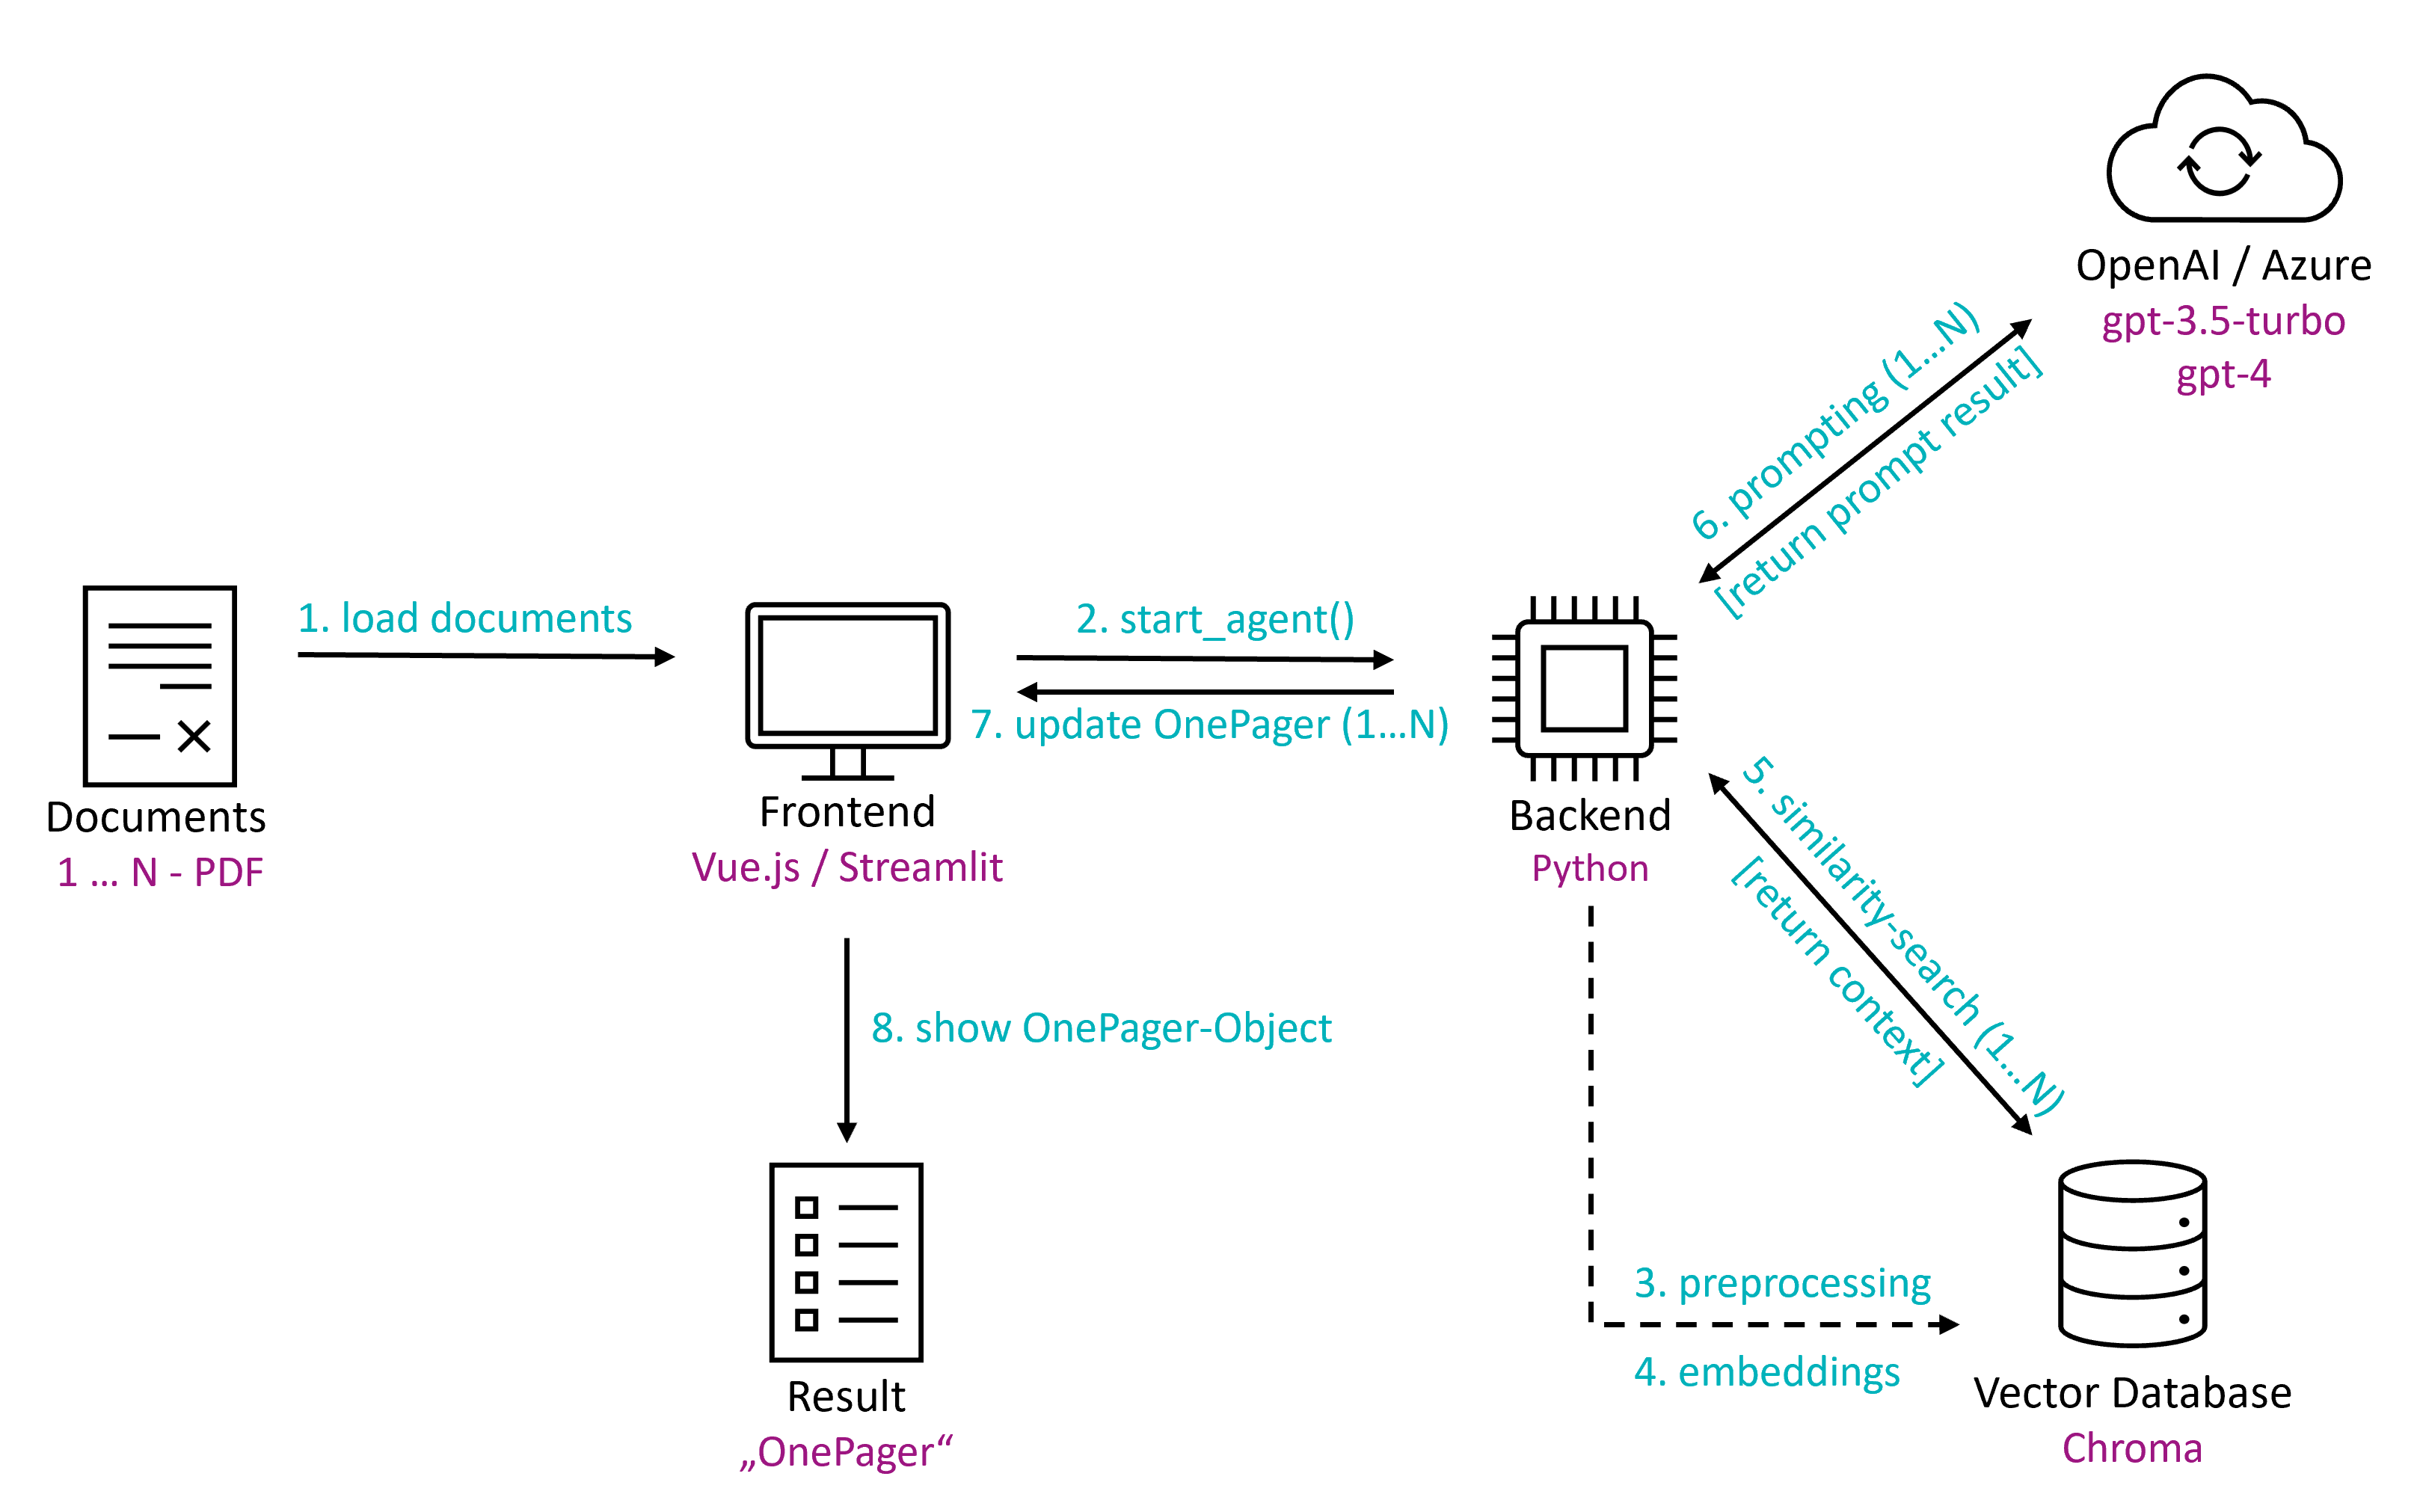
\includegraphics[width=1\textwidth]{figures/DokumentenAgent-Uebersicht.png}
    \caption{Schematische Darstellung der Software-Architektur}
    \label{fig:DokumentenAgent-uebersicht}    % \ref{fig:DokumentenAgent-uebersich}
\end{figure}

Zuerst werden die Ausschreibungsdokumente im Frontend hochgeladen (Siehe 1.) und der Agent wird mit den gewünschten
Prompts gestartet (Siehe 2.). Der Agent beginnt nun im Backend mit dem PreProcessing, welches die Dokumente in fachlich
logische Blöcke aufspaltet und personenbezogene Daten anonymisiert (Siehe 3.). Anschließend wird das Embedding, also
eine Repräsentation der Daten als Vektoren, erstellt und als der Vektordatenbank angelegt (Siehe 4.). Nun wird für jeden
Prompt eine Similarity-Search durchgeführt (Siehe 5.), bei der dem möglichst passende Stellen aus den Dokumenten aus der
Vektordatenbank extrahiert werden, damit diese im Prompt als Kontext eingebettet für die Textvervollständigung an das
LLM übergeben werden (Siehe 6.). Das Ergebnis wird in ein JSON-Objekt übersetzt und der OnePager wird entsprechend
aktualisiert (Siehe 7.). Währenddessen baut sich im Frontend Stück für Stück der OnePager mit allen gefundenen
Informationen zusammen (Siehe 8.).

\section{Meine Rolle und Aufgaben im Projekt}
Ich bin in der Rolle eines Softwareentwicklers in das Projekt gekommen. Meine Aufgabe bestand Anfangs darin, die Prompts
für die einzelnen Felder des One Pagers zu formulieren um die gelieferten Ergebnisse zu verbessern. Dies resultierte in
den Aufbau einer Test- und Evaluierungsarchitektur in Python mithilfe derer die Prompts vollautomatisch bewertet werden
und anhand ihrer Kennzahl ausgewählt und weiter optimiert werden. Durch Komplikationen mit dem Datenschutz wurde der
Umstieg von Langchain auf Azure von Microsoft beschlossen, welchen ich durchgeführt habe. 

\subsection{Prompt Engineering}
Um gute Ergebnisse durch die Textvervollständigung der Sprachmodelle zu erhalten ist es unumgänglich hochwertige Prompts
zu formulieren. Hierfür habe ich mehrere E-Learnings zum Thema \textcite{deeplearning.AI} absolviert, in denen erklärt wird wie
man hochwertige Prompts erstellt und ganze Systeme mit einer Chatbot Integration entwickelt. Besondere Methoden welche im
Projekt zum Einsatz kommen sind Single-Shot-Prompting, bei dem man ein Beispiel gibt wie eine optimale Antwort
auszusehen hat, und die Ausgabe als JSON festzulegen, um die erhaltenen Ergebnisse im Code nutzen und anwenden zu
können. Das Abgrenzen von wichtigen Informationen wie dem mitgelieferten Kontext über sogenannte Delimiter hilft dem
Modell dabei, Aufgabe und Kontext nicht zu vermischen (wenn auch nicht immer perfekt). Gut eignet sich hierfür
'\#\#\#\#', da dies als ein Token zählt und selten regulär vorkommt. Um Halluzinationen, also das produzieren von
Falschinformationen oder ausgedachten Informationen zu vermeiden wird im Prompt explizit darauf hingewiesen, dass bei
nicht vorhandenen Informationen das entsprechende Feld leer gelassen werden soll. 
%Das Bewerten der generierten Antworten durch das Sprachmodell um die Qualität zu messen, welches später im Kapitel
%\ref{chap:Evaluation} Verwendung findet.

\subsection{OnePager}
Der von PMO erstellte OnePager umfasst alle wesentlichen Information der Ausschreibung um eine fundierte Entscheidung
darüber treffen zu können, ob die Ausschreibung als Projekt für iteratec geeignet ist. Informationen sind unter anderem
der Projekttitel, eine kurze Projektbeschreibung, wichtige Termine und Deadlines und Bewertungskriterien. Da jede dieser
Punkte in unterschiedlichen Regionen der Dokumente zu finden ist und die Qualität der Ergebnisse besser ist wenn man
nicht mehrere Fragen in einer Anfrage bündelt wird der OnePager in der Anwendung Frage für Frage zusammengesetzt und
ergänzt. Als Format wird JSON verwendet um später den fertigen OnePager gut speichern und weiterverarbeiten zu können
(zum Beispiel für die Evaluation). Zudem können dem Frontend die Daten so als Variable zur Verfügung gestellt werden.
Die OnePager-Klasse wurde mit vielen Hilfsmethoden ausgestattet um das Arbeiten mit den JSON-Objekten zu erleichtern. Zu
den Hilfsmethoden gehören unter anderem das Initialisieren des OnePager-Template, das Laden und Abspeichern als Datei.
Eine weitere Hilfsmethode ist das Hinzufügen von Teilinformationen aus den einzelnen Ergebnissen des Sprachmodells in
den bestehenden OnePager gehört. Mithilfe von Prüffunktionen werden nicht JSON-Konforme Antworten erkannt um
Maßnahmen (Wiederholen der Anfrage) ergreifen zu können.

\subsection{Verbessern der Kontextauswahl über Similarity Search}
\label{chap:Verbessern der Kontextauswahl über Similarity Search}
Um gezielt die fachlich richtigen Passagen innerhalb des Dokuments zu finden wird eine Query gegen die über das
Embedding generierte Vektordatenbank gestellt. Als Ergebnis erhält man die Textausschnitte, mit der höchsten
Trefferquote. Bei dem eben beschriebenen Verfahren sprechen wir von einer Similarity Search, also dem finden von
ähnlichen Daten innerhalb einer Vektorrepräsentation des bereitgestellten Dokuments. Da es bei Ausschreibungen viele
synonyme Begriffe gibt, welche Informationen zu identischen Fragestellungen geben habe ich diese Begriffe in einem
Lexikon erfasst und gesammelt. Die Akquiseabteilung wurde zusätzlich darum gebeten weitere Ergänzungen vorzunehmen um
fachlich möglichst viele Begriffe abzudecken. Mit dem so erhaltenen Lexikon können wichtige Keywords für die Similarity
Search bereitgestellt werden, vereinzelt wird auch innerhalb der Prompts darauf zurückgegriffen um das Sprachmodell
dabei zu unterstützen die richtigen Informationen der richtigen Stelle des OnePagers zuzuordnen. Über ein Prompt.Config
Dictionary kann nun für jedes Prompt auf entsprechende Felder wie Suchbegriffe, Promptmethode oder Suchergebnisanzahl
individuell zugegriffen werden.

\subsection{Evaluation} 
\label{chap:Evaluation}   
Um festzustellen ob sich Prompts beim Wechsel von Modellen, Promptversionen oder unterschiedlichen
PreProcessing-Verfahren verbessern oder verschlechtern habe ich 10 Testdatensätze aus öffentlichen
Ausschreibungsportalen zusammmengesucht und entsprechende Musterlösungen erarbeitet, sofern dies in unserem fachlichen
Rahmen möglich war. Dies hat uns ermöglicht, ausgewählte Prompts testweise gegen alle 10 Testdatensätze abzufragen.
Hierbei wird die neu generierte Antwort mit der Musterlösung verglichen und anschließend anhand eines Bewertungsschemas
mit Punkten zwischen 0 und 10 inklusive einer Begründung bewertet, je nachdem wie nah das gelieferte Ergebnis an die
Musterlösung herankommt.    

\begin{figure}[h]
    \centering
    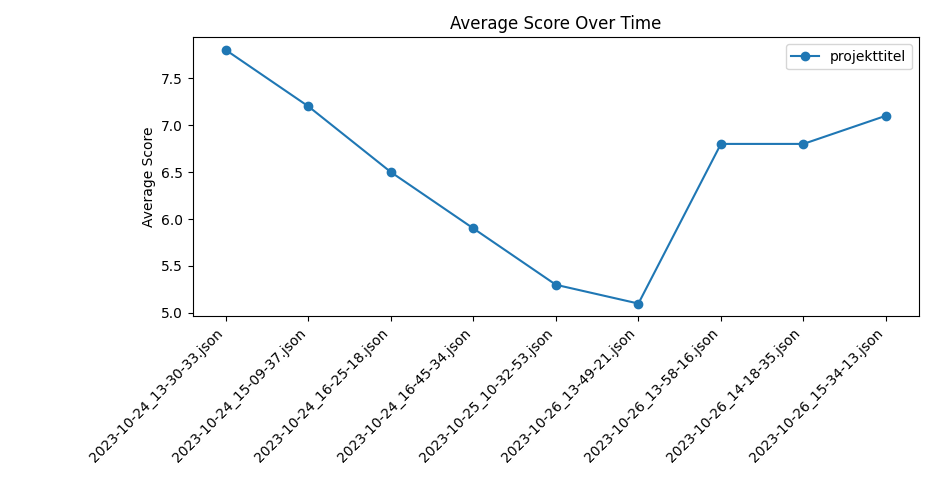
\includegraphics[width=1\textwidth]{figures/02_Prompt_Evaluierung.png}
    \caption{Visualisierung eines Prompts mit verschiedenen Prompt und Bewertungsmodifikationen über Zeit}
    \label{figure:02_Prompt_Evaluierung}     % \ref{figure:02_Prompt_Evaluierung}
\end{figure}

Die einzelnen Punkte werden anschließend für jedes Prompt zu einem Average Score zusammengerechnet und mithilfe der
Visualisierungsklasse als Plot dargestellt. Dabei können einzelne Prompts über verschiedene Versionen und Zeitpunkte
(siehe \ref{figure:02_Prompt_Evaluierung}) oder mehrere Prompts bei Verwendung unterschiedlicher Sprachmodelle
dargestellt und verglichen werden.

% \begin{figure}[h]
%     \centering
%     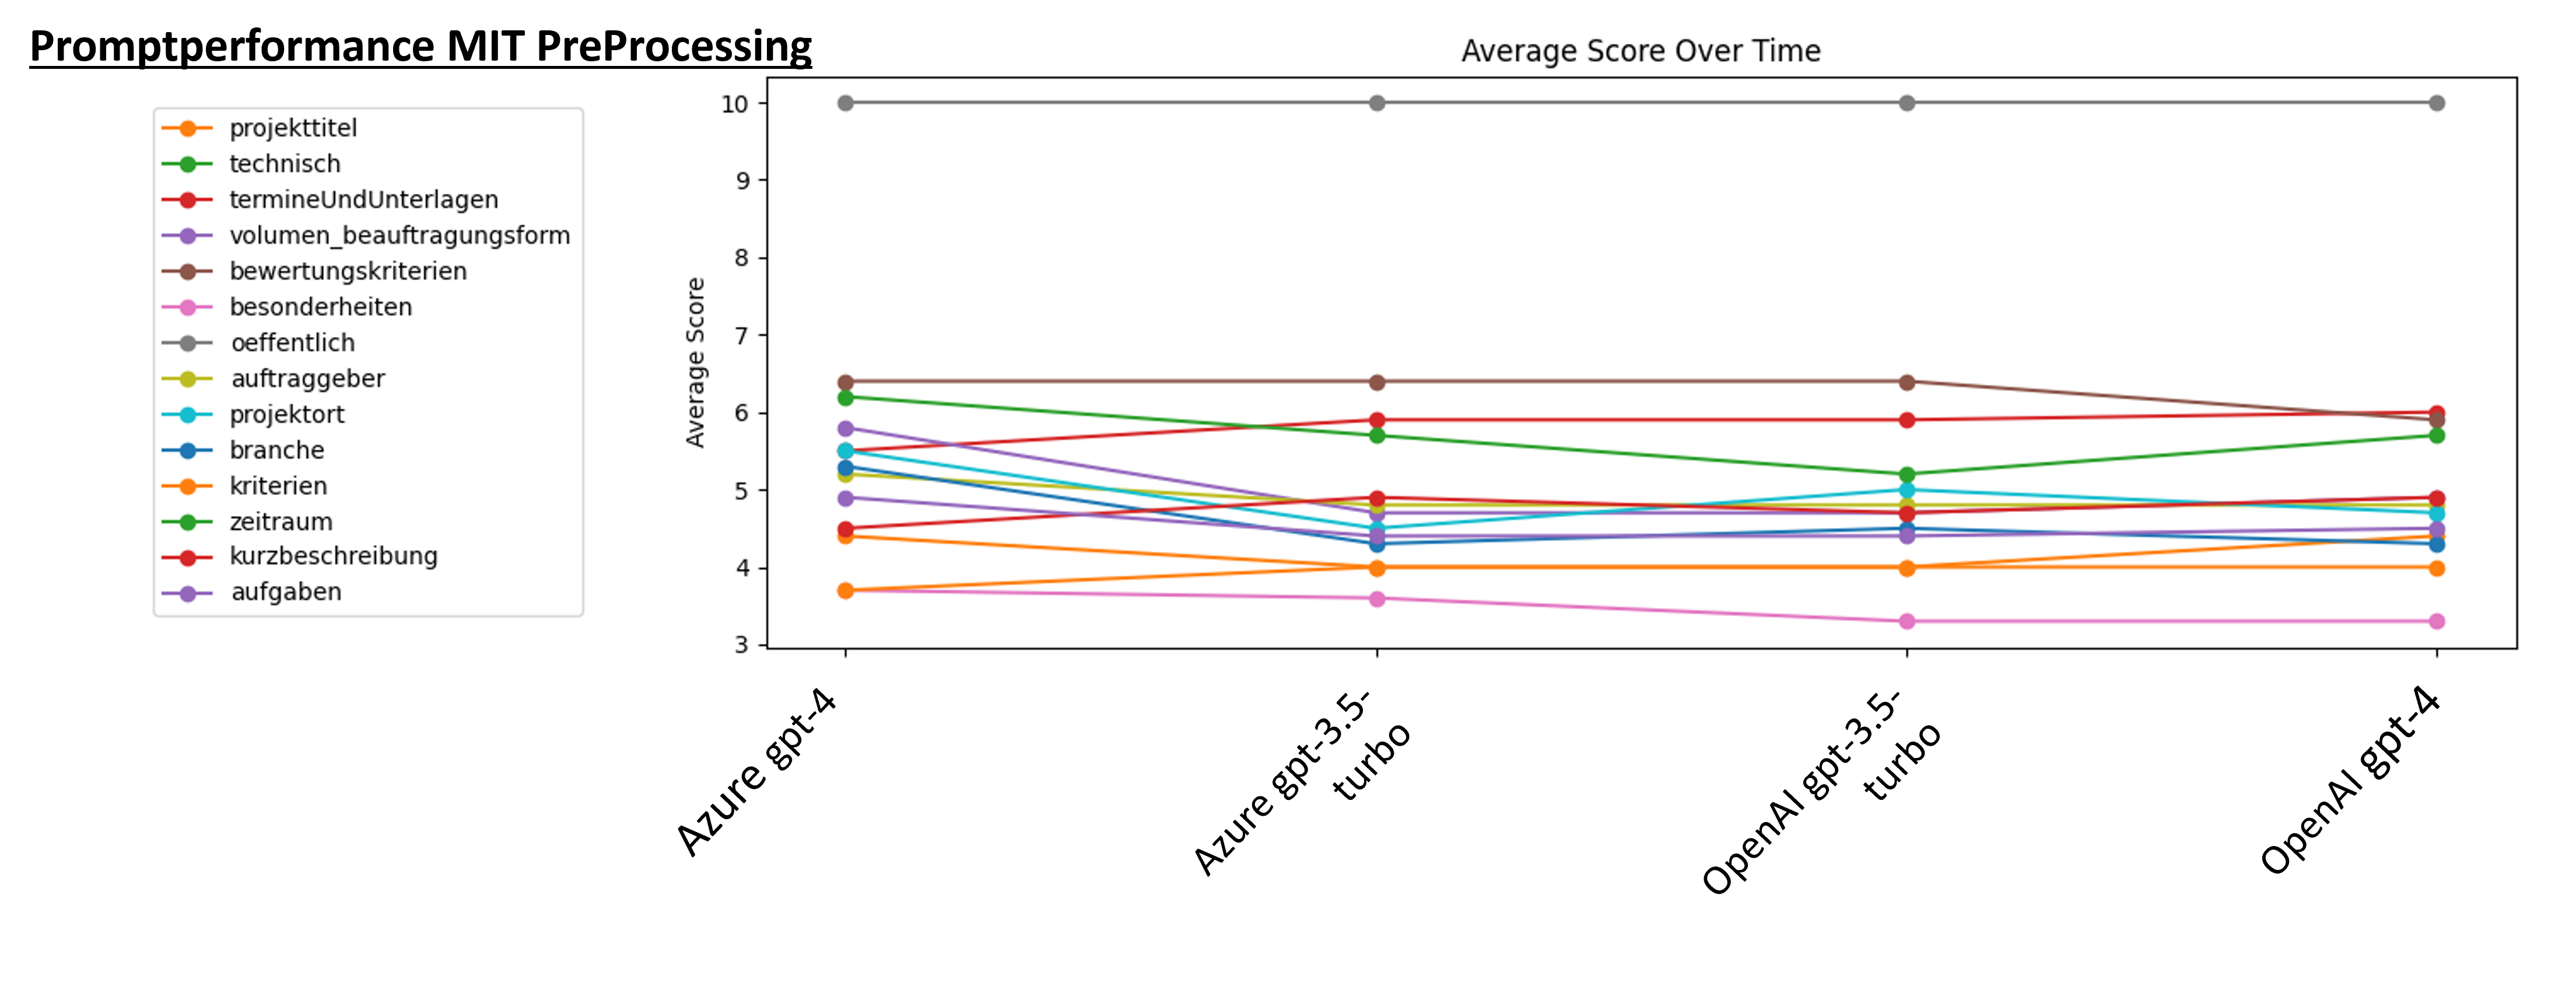
\includegraphics[width=1\textwidth]{figures/04_Prompt_Evaluierung-MitPreProcessing.png}
%     \caption{Visualisierung der Prompts mithilfe unterschiedlicher Modelle. PreProcessing ist aktiviert}
%     \label{fig:04_Prompt_Evaluierung-MitPreProcessing}    % \ref{fig:04_Prompt_Evaluierung-MitPreProcessing}
% \end{figure}

\subsection{Azure Migration}
Die rechtliche Lage bei der Verarbeitung Personenbezogener Daten durch Sprachmodelle wie gpt ist laut unserer
Datenschutzbeauftragten noch sehr unklar solange es noch keine Urteile gibt. Es wurde sich darauf geeinigt auf azure
openAI zu migrieren, da dort europäische Server verwendet werden statt amerikanischer. Ein großer Nachteil von Azure ist
aber, dass man für das Erstellen der Embeddings für die Vektordatenbank auf 16 Inputs beschränkt ist, während openAI
hier keine Einschränkungen vorgibt. Größere Dokumente können leicht auf 1 Input pro Seite kommen, was ein Einbetten von
Dokumenten ab 20 Seiten verhindert. Um das Problem zu lösen habe ich statt die vorgegebene Embedding-Methode zu
verwenden eine eigene Methode erstellt, welche die Dokumente bzw. die Inputs auf mehrere Listen mit einer Größe kleiner
gleich 16 aufteilt. Anschließend werden die einzelnen Listen über eine REST API zu embeddings umgewandelt und wieder
zusammengesetzt. Am ende wird eine Collection mit den Embeddings, den Dokumenten und entsprechenden Metadaten erstellt,
welche zentral in einem VectorDataManager zur Verfügung gestellt wird. Gegen diese Collection können anschließend
Abfragen wie Similarity-Searches (siehe \ref{chap:Verbessern der Kontextauswahl über Similarity Search}) durchgeführt
werden.

\subsection{Dokumentation}
Sämtlicher von mir geschriebener Quellcode wurde mit Ein- und Mehrzeiligen Kommentaren ergänzt, um das Lesen und
Verstehen des Codes zu vereinfachen. Ich habe die gesammelten Erfahrungen in einem Bericht festgehalten und diesen im
Repository abgelegt. Zudem wurden Architecture Decision Records, kurz ADR, erstellt und ebenfalls dem Projekt angehängt.
Diese ADRs sind dazu da, später Einsicht darüber zu geben warum sich für bzw. gegen ein Framework oder eine Technologie
entschieden wurde.

\subsection{Messestand auf der BUILD23}

Zum Abschluss des Projektes wurden wir angefragt, ob wir aufgrund des hohen Interesses an dem Projekt eine Präsentation
während des GS-Meetings und der BUILD23 halten möchten. Das Erstellen der Präsentation und Vortragen dieser gehörte auch
zu meinem Aufgabenbereich.


\section{Herausforderungen und Lösungsansätze}

\subsection{Optimierung der Prompts}
Um die Prompts zu verbessern ist es notwendig, diese an unterschiedlichen Ausschreibungen zu testen und das gelieferte
Ergebnis mit der richtigen Antwort zu vergleichen. Da das größte Dokument über 100 Seiten hat und wir keine
Musterlösungen haben war es schwierig Aussagen über die Qualität der Prompts zu treffen. Die Lösung war das Einführen
einer Metrik welche die Qualität der Prompts misst. Es wurden 10 Dokumente ausgearbeitet und sämtliche wichtige
Informationen in OnePager-JSON Dateien gespeichert. Anschließend wurde eine Testarchitektur geschaffen, in welcher man
die gewünschten Prompts vollautomatisiert gegen die 10 Testdokumente abfragt und anschließend die Resultate zusammen mit
der Musterlösung von ChatGPT auf inhaltliche Übereinstimmung überprüfen und bewerten lässt.

Aus den generierten Bewertungen lassen sich Aussagekräftige Kennzahlen generieren. Zur Darstellung wurde eine
Visualisierungsklasse geschrieben, welche die Punktzahl der Prompts graphisch darstellt (siehe
\ref{fig:03_Prompt_Evaluierung}) und so schnell erkennbar ist, ob der aktuelle Prompt zu einer Verbesserung oder
Verschlechterung der Ergebnisse führt.

\begin{figure}[hbt]
    \centering
    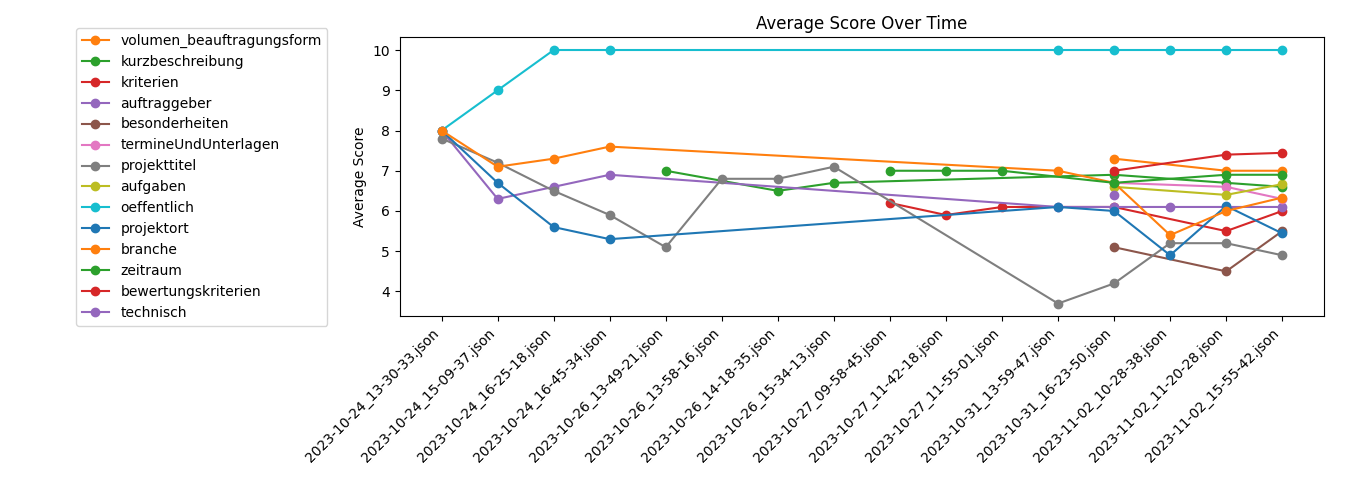
\includegraphics[width=1\textwidth]{figures/03_Prompt_Evaluierung.png}
    \caption{Visualisierung der durchschnittlichen Promptqualität im Laufe der Zeit}
    \label{fig:03_Prompt_Evaluierung}    % \ref{fig:03_Prompt_Evaluierung}
\end{figure}

\subsection{Datenschutz}
Das Übermitteln und verarbeiten von Personenbezogenen Daten ist in Deutschland nur mit Ausdrücklicher Genehmigung der
entsprechenden Person zulässig. Laut unserer Datenschutzbeauftragten ist unklar inwiefern das Übermitteln der Daten aus
den Dokumenten über die OpenAI API hierunter einzustufen ist. Da die Server von OpenAI allerdings in den USA liegen
gestalten sich Probleme mit europäischem Datenschutzrecht. Als Lösung wurde die Umstellung auf Azure in Betracht
gezogen, da die Server auf europäischem Boden stehen und damit zumindest nach europäischem Recht Datenschutzkonform
sind. Zusätzlich anonymisieren wir so gut wie alle Personenbezogenen Daten bevor wir diese an das Sprachmodell
übermitteln, indem wir den Kontext vor gegen eine Liste mit allen möglichen Vor- und Nachnamen prüfen, 
und so Namen und Mailadressen herausfiltern.


\section{Ergebnisse und Erfahrungen}

\subsection{Proof of Concept}

Der PoC ist in der Lage viele der gesuchten Informationen aus den Dokumenten zu extrahieren und grafisch für den Nutzer
aufzubereiten. Allerdings fehlen oft Teilinformationen oder es werden Halluzinationen bzw. Falschinformationen
hinzugefügt. Ein möglicher Grund hierfür sind eventuell das PreProcessing,welches aufgrund der limitierten Kontextgröße
von gpt-3.5 und gpt-4 notwendig ist. Durch neue Modelle, wie dem gegen Ende des Projekts angekündigten
\textcite{gpt-4-turbo}, welches eine Kontextlänge von 128K Tokens besitzt, wird man nicht länger gezwungen sein sich auf
kleine Textausschnitte zu begrenzen. Man kann ganze Kapitel übergeben und Limitierungen haben mehr wirtschaftliche
Gründe als Technische. Auch die Fehleranfälligkeit wird durch einen eingebauten JSON-Parser weiter sinken. Unsere Tests
zeigen keine Nennenswerte Unterschiede zwischen den Modellen gpt-3.5-turbo und gpt-4 was die Qualität der Prompts
angeht. Der Versuch hat gezeigt, dass die Grundfunktionen, das übergeben von Ausschreibungsdokumenten und deren Analyse
mithilfe eines Sprachmodells zur automatisierten Erstellung eines OnePager, technisch definitiv möglich sind. Wichtig
für die Zukunft ist jedoch es Klarheit beim Umgang mit Personenbezogenen Daten im Zusammenhang mit Sprachmodellen zu
schaffen und gegebenenfalls eine geeignete Filterung dieser Daten zu implementieren.

\subsection{Persönlich}
Persönlich konnte ich in dem Projekt lernen, wie man mithilfe eines Jira-Boards als Gruppe iterativ Software entwickelt.
Ich habe mit Python eine neue Programmiersprache gelernt, welche vielseitig einsetzbar ist und vor allem im Bereich der
Künstlichen Intelligenz und Machine Learning viele Möglichkeiten bietet. Zudem konnte ich ein tieferes Verständnis für
Prompts und deren Einsatzmöglichkeiten aufbauen. Das Entwickeln einer ganze Applikation, welche Sprachmodelle oder
andere LLMs integriert ist für mich nun verständlich und durchführbar. Ich konnte auch Erfahrungen im Dokumentieren von
Entwicklungsartefakten und Entscheidungen sammeln, welche sich in zukünftigen Projekten weiter vertiefen lassen. 
    \chapter{TenderSniffer}

\section{Kurze Projektbeschreibung}
TenderSniffer ist ein Projekt, welches aus mehreren Applikationen besteht und zum Ziel hat verschiedene
Ausschreibungsportale nach neuen Ausschreibungen zu durchsuchen und die gefundenen Ausschreibungen visuell strukturiert
darzustellen. Teilanwendungen hierbei sind der TenderCrawler, welcher die Ausschreibungen von den einzelnen Plattformen
zieht und in die Datenbank speichert. Der TenderWeb ist ein Graphisches User Interface (GUI), welches die
Ausschreibungen in der Datenbank darstellt und Benutzereingaben abspeichert. Mithilfe von verschiedenen Schaltflächen
kann die Ausschreibung entweder an die Akquiseabteilung weitergeleitet werden oder für unpassend deklarieren.

\section{Verwendete Software und Grundlagen}
In diesem Kapitel werden alle SW-Werkzeuge und Technologien beschrieben, welche im Entwicklungsumfeld des TenderSniffers
verwendet werden oder für ein Verständnis zuträglich sind.

\subsection{Werkzeuge}

\subsubsection{IntelliJ IDEA}
Integrierte Entwicklungsumgebung des Softwareunternehmens JetBrains. Wird für die Entwicklung mit Java und Kotlin
eingesetzt. 

\subsubsection{PostgreSQL}
Freies Datenbankmanagementsystem, welches seit 1997 von einer Open-Source-Community weiterentwickelt wird. Es wird oft
mit Postgres abgekürzt.

\subsubsection{SonarQube}
Plattform für statische Analyse und Bewertung von Quelltext. Die Ergebnisse der Analyse werden über eine Website dargestellt.

\subsubsection{Lint}
Werkzeug, welches den Quellcode auf Fehler, unübliche Muster, nicht eingehaltene Stilrichtlinien und potenzielle Bugs
überprüfen, um eine bessere Codequalität und -konsistenz zu gewährleisten.


\subsection{Technologien}

\subsubsection{Java}
Java ist eine objektorientierte höhere Programmiersprache welche 2010 von Oracle übernommen wurde.
Sie findet neben Computerapplikationen auch Einsatz bei Apps für Smartphones, Tablets und Spielekonsolen.

\subsubsection{JavaScript}
JavaScript ist eine vielseitige und weit verbreitete Programmiersprache, die hauptsächlich für die Entwicklung von
interaktiven Webseiten und Webanwendungen eingesetzt wird.

\subsubsection{Spring Boot}
Spring Boot ist ein Java-Framework zur Vereinfachung der Entwicklung und Bereitstellung von Spring-basierten
Anwendungen, das auf Konvention statt Konfiguration setzt und zahlreiche Funktionen für einen schnellen Projektstart
bietet.

\subsubsection{Vue.js}
Vue.js ist ein JavaScript-Framework, das für den Aufbau interaktiver Web-Oberflächen und Single-Page-Applikationen verwendet wird.

\subsubsection{Jest}
Jest ist ein JavaScript-Test-Framework, das für seine einfache Konfiguration und effiziente Leistung bei der Entwicklung
von Webanwendungen bekannt ist.

\section{Meine Rolle und Aufgaben im Projekt}
Ich bin in der Rolle eines Softwareentwickler zum Projekt hinzugestoßen, es wird agil mithilfe von Jiraboards und
Sprints entwickelt. Ein Sprint geht über vier Wochen, da ein großteil der Projektbeteiligten Werkstudenten sind und
entsprechend nur ein bis zwei Tage pro Woche arbeiten. Die Endnutzer (PMO- und Akquiseabteilungen) erstellen
eigenständig neue tickets und beschreiben darin aus Benutzersicht welche Funktionen, Änderungen und Fehler gewünscht
sind, bzw. beseitigt werden sollen. Neben den täglichen Austauschterminen, den sogenannten "Dailies" gibt es jeden
Freitag einen größeren Besprechungstermin, die "Weeklies". Am ende eines jeden Sprints findet ein "Review", bevor der
nächste Sprint begonnen wird.

\subsection{Kommentare ausblenden}
Meine Einstiegsaufgabe war es in der Kommentarsektion einen Button im Frontend des TenderWeb zu programmieren, mit dem
der Kommentarbereich eingeklappt werden kann sobald dieser mehr als 3 Kommentare enthält. Hierfür habe ich die
vorhandene commentBox.vue um den besagten button erweitert und mithilfe von javascript die Logik hinter dem button
implementiert. Nach mehreren Schleifen mit dem Team und den Nutzern habe ich für die finale Version tests mithilfe von
jest geschrieben. Im Anschluss habe ich den Merge Request erstellt und nachdem die DevOps Pipeline erfolgreich
durchgelaufen ist und die Funktion auf dem Testbuild einwandfrei funktioniert hat wurde das Feature auf der
Produktionsumgebung ausgeliefert und das Ticket abgeschlossen.

\subsection{Auftraggeberdetails erfassen}
Die zweite und umfangreichste Aufgabe war es, die Daten der Auftraggeber in einer eigenen Box anzuzeigen und editierbar
zu gestalten, so dass Änderungen konsistent sind. Hierfür habe ich das Datenbankschema um eine client-tabelle erweitert
und im Backend entsprechende domain-, repository-, service- und Controllerklassen geschrieben, mit denen über HTTP
Requests die API angesprochen werden kann und Auftaggeber sowohl abgerufen als auch gespeichert werden können. Im
Frontend habe ich den store, welcher als zentraler Ort zur Speicherung und Verwaltung des Anwendungszustands, was eine
konsistente Datenverwaltung und -verteilung über die gesamte Anwendung hinweg ermöglicht, um entsprechende Methoden
erweitert. Anschließend habe ich eine clientBox mit vue erstellt, welche diese Daten aus dem store anzeigt und bei
Änderungen mithilfe von store Mutationen und Aktionen die neuen Daten über eine POST Request an das Backend übermittelt
und somit konsistent in der Datenbank abgespeichert werden. 



    %\chapter{Reflexion und Bewertung}


\section{Persönliche Reflexion über das Praxissemester}

Persönliche Reflexion über das Praxissemester: Was hast du gelernt? Welche Fähigkeiten konntest du verbessern?

\section{Bewertung der Zusammenarbeit im Team und im Unternehmen}

\section{Einordnung der erlernten Inhalte und Fähigkeiten im Kontext deines Studiums}

    \chapter{Fazit und Ausblick}


\section{Zusammenfassung der wichtigsten Erkenntnisse}
Im Praktikum konnte ich meine Kenntnisse über KI und deren Integration in Softwareprojekte umfassend erweitern. Das
arbeiten mit Kollegen im Team so wie das Entwickeln agiler Software mithilfe von Scrum waren eine erfrischende und
spannende Abwechslung. Ich habe für mich viel dazugelernt, auch abseits des Schreibens von Quellcode habe ich gelernt
wie man wichtige Entscheidungen und Erkenntnisse festhält und dokumentiert, wie man neue Technologien einsetzt und auch
wie man Software plant und veröffentlicht.


\section{Einordnung der erlernten Inhalte und Fähigkeiten im Kontext deines Studiums}
Meine Programmierkenntnisse aus Programmieren 1 und 2 konnte ich beim Programmieren mit Java und Javascript einsetzten und beim
Programmieren mit Python erweitern. Bei der Anpassung der Datenbank im TenderSniffer waren die gelernten Inhalte über
relationale Datenbanken aus dem Modul Datenbanken sehr hilfreich. Am meisten profitiert habe ich neben dem Wissen aus
Programmieren 1 und 2 von Software-Technik, da mich hier besonders viele Themen abseits von Quellcode schreiben auf
meine Arbeit als Softwareentwickler vorbereitet haben. Dazu gehören Versionskontrollen wie Git, Softwareentwicklungsmodelle wie Scrum und
Kanban, aber auch DevOps Themen wie CI/CD Pipelines und das Testen von Code.


\section{Weiterer Werdegang}
Meine Erfahrungen im Praxissemester haben mich darin bestätigt meine berufliche Zukunft im Bereich der
Softwareentwicklung zu gestalten. Ich habe viel Freude daran Software zu entwickeln und im Team an Lösungen zu arbeiten. 
Eine berufliche Zukunft bei iteratec kann ich mir sehr gut vorstellen, da die Arbeitsbedingungen durch einen hohen Grad
an Betreuung und Flexibilität, sowie die unfassbar freundlichen und sympathischen Kollegen für eine leistungsorientierte
aber zugleich sehr harmonische Arbeitsatmosphäre sorgen in der ich mich sehr wohl gefühlt habe.
    % \chapter{Anhang}
Eventuell Codebeispiele, Diagramme, Screenshots oder sonstige unterstützende Materialien, die im Hauptteil zu umfangreich wären.

\section{Literaturverzeichnis}

https://www.deeplearning.ai/short-courses/building-systems-with-chatgpt/
    % \chapter{Eidesstattliche Erklärung}
Bestätigung, dass du den Bericht selbstständig verfasst hast (sofern von deiner Hochschule gefordert).
    % \chapter{Zusammenfassung und Ausblick}
Im letzten Kapitel sollte die Arbeit zusammengefasst und ein Fazit gezogen werden. Außerdem sollte beschrieben werden, wie es mit dem Projekt weitergehen kann und welche Punkte vielleicht interessant wären aber im Rahmen der Arbeit nicht bearbeitet werden konnten.

    % diese Zeilen auskommentieren, um das Tutorial aus der Arbeit auszublenden.
    %\chapter{Tutorial zu dieser LaTeX-Vorlage}
Dieses Kapitel ist spezifisch für die \LaTeX Vorlage und sollte natürlich in der finalen Abgabe nicht enthalten sein.
Dieser Teil der Arbeit kann bei Bedarf durch einen Kommentar einfach ausgeblendet werden (siehe thesis.tex Zeile 125).






\section{Verwendung dieser Vorlage}
Dieses Template ist für die Verwendung mit pdflatex gedacht. Am einfachsten ist es die Vorlage in Overleaf \cite{overleaf} zu öffnen. Overleaf ist eine Onlineanwendung zum Arbeiten mit \LaTeX{}, was den Vorteil hat, dass nichts lokal installiert werden muss und mit jedem Betriebssystem gearbeitet werden kann, das über einen Browser verfügt. Außerdem ist es möglich mit mehreren Personen gemeinsam an einem Projekt zu arbeiten. Die Vorlage kann auch mit einer lokalen Installation verwendet werden. Die Website von Overleaf bietet zudem einige gute Tutorials zum Arbeiten mit \LaTeX{}: \url{https://www.overleaf.com/learn}.

Fehler und Warnungen, die beim Compilieren erzeugt werden, sollten direkt behoben werden, da es später schwierig sein kann den eigentlichen Auslöser einer Fehlermeldung zu finden. Manchmal sieht das Dokument trotz Fehlermeldung oder Warnung korrekt aus, der Fehler macht sich dann aber später bemerkbar. Die Meldungen sind leider oft nicht sehr aussagekräftig, weshalb es am einfachsten ist direkt nach dem Auftreten eines Fehlers den Teil der Arbeit anzuschauen, der als letztes geändert wurde.

\section{Projektstruktur}

Der Hauptteil einer Thesis besteht üblicherweise aus mehreren Kapiteln, die verschiedene Aspekte der Arbeit beleuchten. 
Es ist ratsam für jedes Kapitel ein eigene Tex-Datei anzulegen, damit der Quellcode übersichtlich bleibt. Durch einen numerischen Präfix (z.B.: \texttt{20\_relatedwork.tex} siehe Abb. \ref{fig:folderstructure}) werden die Quelldateien in der richtigen Reihenfolge in Overleaf angezeigt. Wir verwenden 20 anstatt 2, damit wir nachträglich auch noch 21, 22, etc. einfügen können.

\begin{figure}
    \centering
    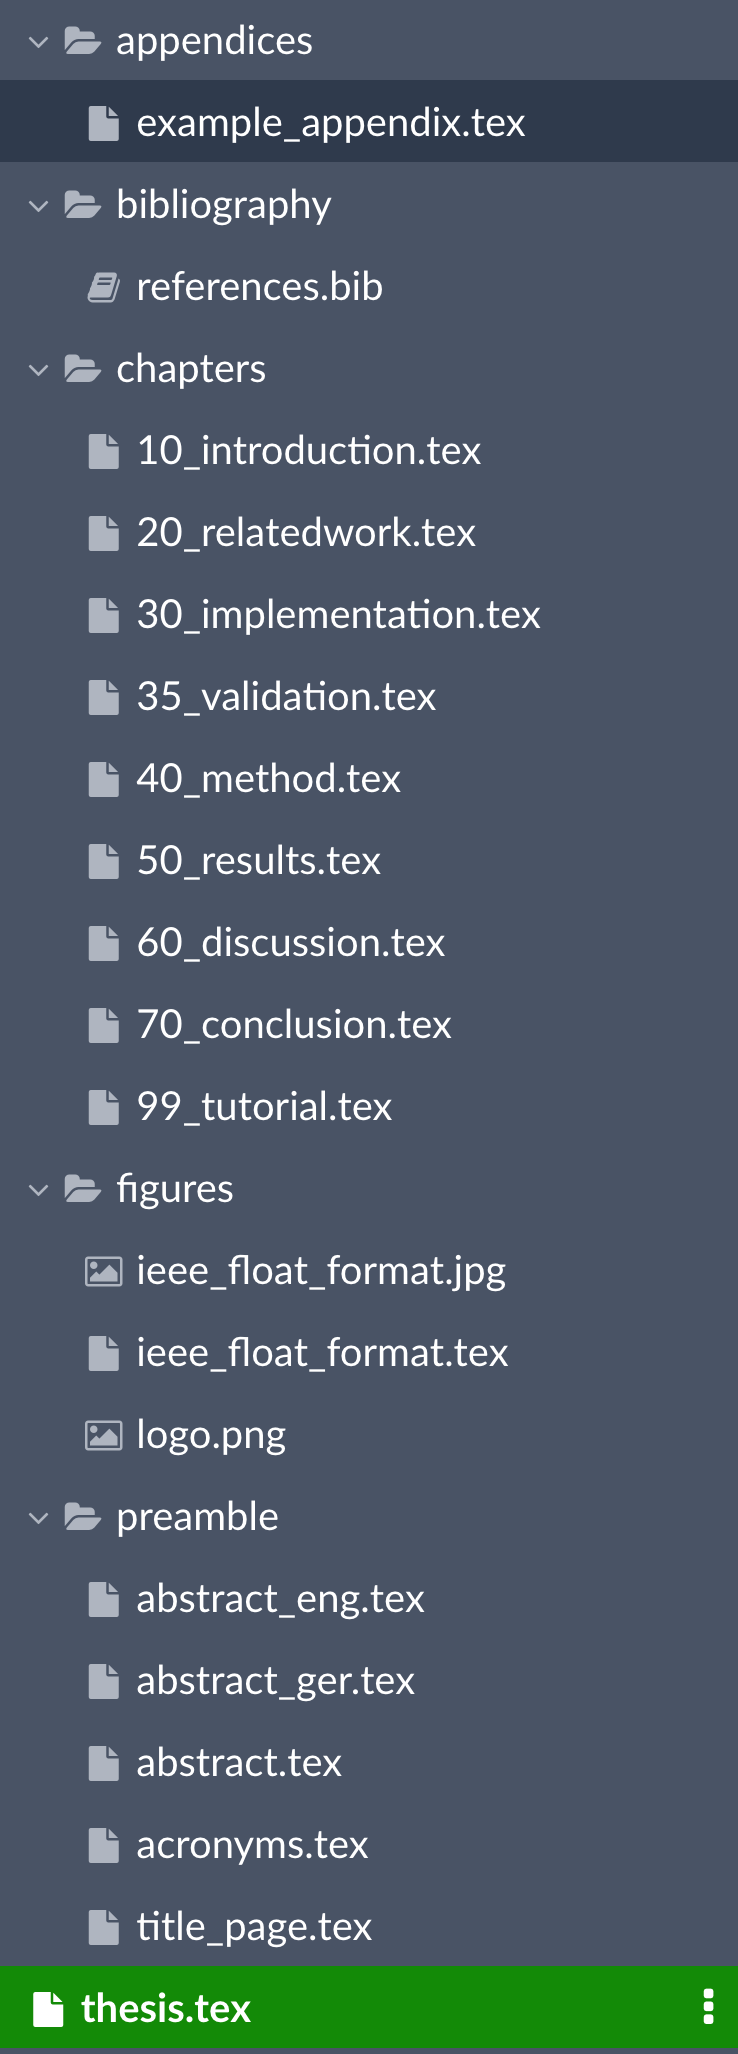
\includegraphics[width=0.4\linewidth]{figures/folderstructure.png}
    \caption{Ordnerstruktur eines LaTeX-Projektes}
    \label{fig:folderstructure}
\end{figure}

\subsection{Unterkapitel}
Unterkapitel sollten ein abgeschlossenes Thema behandeln. Einzelne Unterkapitel in einem Kapitel sind zu vermeiden, also z.\,B. in Kapitel 2 das Unterkapitel 2.1, aber kein weiteres Unterkapitel. In diesem Fall ist es besser entweder den Inhalt von 2.1 direkt in Kapitel 2 zu schreiben, oder falls 2 und 2.1 thematisch zu weit voneinander entfernt sind, aus Unterkapitel 2.1 ein eigenes Kapitel 3 zu machen. Dieses Unterkapitel ist ein negativ Beispiel dafür. 

\section{Grafiken}
In der Informatik sind die häufigsten Grafiken entweder Diagramme oder Plots. Beide Arten von Grafiken lassen sich gut als Vektorgrafiken erstellen und einbinden. Der Vorteil von Vektor- gegenüber Pixelgrafiken ist, dass beliebig weit in eine Grafik hereingezoomt werden kann, ohne dass sie unscharf wird. Zudem benötigen Vektorgrafiken meistens weniger Speicherplatz.

\subsection{Vektor- vs Pixelgrafiken}
Für die meisten Abbildungen sollte man Vektorgrafiken verwenden, diese können verlustfrei skaliert werden und bieten somit die meisten Freiheiten.
Wenn man Grafiken in R erstellt, können die Plots als pdf oder svg-Dateien abgespeichert werden und liegen dann ebenfalls als Vektorgrafik vor. Ein weiteres beliebtes Programm zum Erstellen von Vektorgrafiken ist Inkscape \cite{inkscape}. Zudem bieten viele Programme die Möglichkeit eine Grafik z.\,B. als PDF zu exportieren, was in \LaTeX{} als Vektorgrafik eingebunden werden kann. Adobe Indesign wird auch häufig zum Erstellen von Vektorgrafiken verwendet.

\paragraph{Profi-Tipp TikZ.}
Grafiken können direkt in \LaTeX{} mit dem TikZ Paket \cite{tikz} erstellt werden. Die Verwendung ist etwas gewöhnungsbedürftig, da Grafiken mit Code beschrieben werden, bietet aber viele Freiheiten. Außerdem werden die so erstellten Grafiken direkt in \LaTeX{} gerendert und verwenden die selbe Schriftart wie im Text und eine konsistente Schriftgröße im gesamten Dokument. 

Pixelgrafiken lassen sich nicht immer vermeiden, z.\,B. wenn eine Foto in die Arbeit eingebunden werden soll. In diesem Fall sollte darauf geachtet werden, dass die Grafik über eine ausreichende Auflösung verfügt. Eine Auflösung von 300~dpi ist ein guter Richtwert, um beim Drucken ein gutes Ergebnis zu erhalten.

Abbildungen \ref{fig:ieee_float_format_vector} und \ref{fig:ieee_float_format_pixel} zeigen beide den Aufbau des IEEE Floating Point Formats. Abbidlung \ref{fig:ieee_float_format_pixel} ist eine Pixelgrafik, während Abbildung \ref{fig:ieee_float_format_vector} mit TikZ erstellt wurde. Der Unterschied wird beim hereinzoomen deutlich.

\begin{figure}[ht]
\centering
% Beispiel für eine mit TIKZ erstellte Grafik

\begin{tikzpicture}
[node distance=0cm]
\tikzset{rectangle_black/.style = {rectangle, minimum width=1cm, minimum height=0.75cm, text centered, draw=black, fill=white}};
\tikzset{rectangle_white/.style = {rectangle, minimum width=1cm, minimum height=0.75cm, text centered, draw=none, fill=none}};
\node (sign) [rectangle_black] {S (sign)};
\node (exponent) [rectangle_black, right = of sign] {E (biased exponent)};
\node (fraction) [rectangle_black, right = of exponent] {T (trailing significand field)};
\node (sign_text) [rectangle_white, above = of sign] {1};
\node (exponent_text) [rectangle_white, above = of exponent] {$w$};
\node (fraction_text) [rectangle_white, above = of fraction] {$t=p-1$};
\node (bits) [rectangle_white, above = of fraction, right = of fraction_text] {bits};

\end{tikzpicture}

\caption{Aufbau des IEEE Floating Point Formats als Vektorgrafik mit TikZ erzeugt.}
\label{fig:ieee_float_format_vector}
\end{figure}

\begin{figure}[ht]
\centering
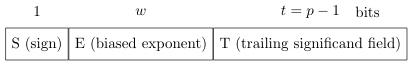
\includegraphics[width=0.65\textwidth]{figures/ieee_float_format.jpg}
\caption{Aufbau des IEEE Floating Point Formats als Pixelgrafik.}
\label{fig:ieee_float_format_pixel}
\end{figure}

\section{Tabellen}
Tabellen können in \LaTeX{} direkt erstellt werden. Tabelle \ref{tab:ieee_formats} zeigt ein Beispiel dafür. Einfache Tabellen lassen sich schnell erstellen, bei komplizierteren Tabellen ist es manchmal einfacher zusätzliche Pakete zu verwenden. Mit dem Paket \texttt{multirow} können z.\,B. einfacher Tabellen erstellt werden, bei denen einzelne Zeilen oder Spalten zusammengefasst sind. 

Unter \url{https://www.tablesgenerator.com/} findet man ein hilfreiches online Werkzeug zum erstellen von Tabellen. Wichtig ist es hier den \textquote{Default table style} zum \textquote{Booktabs table style umzustellen}. 

\begin{table}[ht]
\centering
\begin{tabular}{lrrrr} 
 \toprule
 Parameter & binary16 & binary32 & binary64 & binary128 \\
 \midrule
  $k$, storage width in bits           & 16 &  32 &   64 &   128 \\ 
  $w$, exponent field width in bits    &  5 &   8 &   11 &    15 \\
  $t$, significand field width in bits & 10 &  23 &   52 &   112 \\
  emax, maximum exponent $e$           & 15 & 127 & 1023 & 16383 \\
  bias, $E-e$                          & 15 & 127 & 1023 & 16383 \\
 \bottomrule
\end{tabular}
\caption{IEEE 754-2019 Floating Point Formate als Beispiel für das Einbinden einer Tabelle.}
\label{tab:ieee_formats}
\end{table}

\section{Quellcode}
Um Quellcode in die Arbeit einzubinden, können in \LaTeX{} Listings verwendet werden. Es gibt für populäre Sprachen vorgefertigte Umgebungen, welche die Syntax farblich hervorheben. Quellcode sollte eingebunden werden, wenn eine konkrete Implementierung in einer Sprache erläutert wird. Für die Erklärung eines Algorithmus ist es oft übersichtlicher ein Schaubild oder Pseudocode zu verwenden. Es sollten nur kurze Codeabschnitte eingebunden werden, die für den Leser einfach nachvollziehbar sind und nur den für die Erklärung relevanten Code enthalten. Längere Codeabschnitte können im Anhang stehen. Der komplette Code, der für die Arbeit geschrieben wurde, sollte in einem Repository (Gitlab) % oder Github)
abgelegt werden.

Listing~\ref{lst:example_listing} zeigt ein Beispiel für ein Codelisting in der Programmiersprache C. Algorithmus \ref{alg:west} zeigt einen Routing Algorithmus als Pseudocode. Der Code wurde mit dem Paket algorithm2e \cite{algorithm2e} erstellt.

\begin{lstlisting}[language=C, caption=Beispiel für ein Codelisting in der Sprache C., label=lst:example_listing]
#include <stdio.h>
// comments are highlighted in green
void main() {
    // keywords of the language are highlighted in blue
    for (int i = 0; i <= 42; ++i) {
        printf("%d\n", i);
    }
    // strings are highlighted in red
    printf("Hello World!");
}
\end{lstlisting}

\begin{algorithm}[ht]

    \uIf{destination in west direction}{
        go West;
    }
    \uElseIf{destination in same column}{
        \eIf{destination in north direction}{
            go North;
        }{
            go South;
        }
    }
    \uElseIf{destination in north east direction}{
        go North or go East
    }
    \uElseIf{destination in south east direction}{
        go South or go East
    }
    \uElseIf{destination in same row and in east direction}{
        go East;
    }
    \uElseIf{at destination}{
        done;
}
 \caption{West First-Routing Algorithm.}
 \label{alg:west}
\end{algorithm}

\section{Literatur}
Ein Literaturverzeichnis sollte mit dem apa Paket für BibLatex erstellt werden. Dazu wird für jede Quelle ein Eintrag in der Datei \texttt{references.bib} angelegt. An der passenden Stelle im Text können diese Einträge mit dem \texttt{\textbackslash cite\{\}} Befehl zitiert werden. Für jede Quelle die zitiert wird, legt \LaTeX{}  im Literaturverzeichnis einen Eintrag an.

Beschreibungen der Quellen im Bibtex-Format müssen meistens nicht selbst erstellt werden, sondern können direkt bei vielen Verlagen und Bibliotheken direkt generiert werden. Google bietet mit dem \textquote{Scholar-Button} ein Chromium Plugin, mit dem schnell bibtex-Einträge generiert werden können. Bei Google-Scholar generierten Bibtex-Einträgen muss auch eine manuelle Endkontrolle stattfinden, um zu prüfen, ob die Daten in Google korrekt gespeichert waren (z.B.~fehlende Autoren, falsche Jahreszahl, etc.).

Es gibt verschiedene Arten wie man mit biblatex zitiert.\\
\noindent
\texttt{\textbackslash autocite\{valdez2015reducing\}} führt zu \autocite{valdez2015reducing}.\\
\texttt{\textbackslash parencite\{valdez2015reducing\}} führt zu \parencite{valdez2015reducing}.\\
\texttt{\textbackslash textcite\{valdez2015reducing\}} führt zu \textcite{valdez2015reducing}.\\
\texttt{\textbackslash cite\{valdez2015reducing\}} führt zu \cite{valdez2015reducing}.\\
\texttt{\textbackslash autocite[siehe auch][S. 13]\{valdez2015reducing\}} führt zu \autocite[siehe auch][S.~13]{valdez2015reducing}.\\

Hier\footnote{\url{https://tug.ctan.org/info/biblatex-cheatsheet/biblatex-cheatsheet.pdf}} gibt es ein hilfreiches Cheat-Sheet.

Je nach zitierter Dokumentsorte, sieht die Referenz im Literaturverzeichnis anders aus.
\begin{itemize}
    \item Beispiel für einen Konferenzbeitrag \autocite{Nielsen1990}
    \item Beispiel für einen Journal-Artikel \autocite{hollan2000}
    \item Beispiel für ein Buch~\autocite{zobel2014writing}.
    \item Beispiel für eine Norm~\autocite{ISO9241}.
    \item Beispiel für einen Weblink\footnote{{\url{http://imis.uni-luebeck.de}} \autocite{webimis}}

\end{itemize}


\section{Abkürzungen}
Für jede verwendete Abkürzung kann ein Eintrag in der Datei \texttt{acronyms.tex} angelegt werden. Wenn diese Abkürzung im Text zum ersten Mal auftaucht, sollte der Begriff ausgeschrieben werden mit der Abkürzung in Klammern dahinter. Bei weiteren Vorkommen im Text kann dann die eigentliche Abkürzung verwendet werden. In \LaTeX{} gibt es dafür spezielle Befehle. Beispiel für ausgeschriebene Abkürzung (siehe Quelltext des Dokuments für die entsprechenden Befehle).

Erste Verwendung mit Erläuterung: \acrfull{nic}.\\ 
Beispiel für das Verwenden der Abkürzung: \acrshort{nic}. 

Die verwendeten Abkürzungen werden automatisch im Abkürzungsverzeichnis aufgelistet.



    %

\section{LaTeX Eigenarten}
Hier noch ein paar latexspezifische Dinge beim Schreiben.

\paragraph{Non-Breaking Space.}
Mit dem Tildezeichen $\sim{}$ bekommt man ein sog. non-breaking Space~(nbsp). Das ist hilfreich, wenn man verhindern möchte, dass z.B. die Zeile mit einer Referenz beginnt (Beispiel: Listing~\ref{lst:example_listing} -- Hier wird Listing niemals von der Zahl getrennt werden).
Das nbsp wird auch verwendet, um den Abstand nach einem Punkt in einer Abkürzung (1 Einheit) nicht auf die Länge des Abstandes nach dem Satzende zu setzen (1,5 Einheiten). Das fällt nicht immer jedem auf, wenn man es aber einmal sieht, kann man es schwer wieder abschalten.\\
Beispiel: Dies ist eine Abk.~in einem Satz. (korrekt) Die Leertaste wird hier immer gleich lang gehalten.\\
Beispiel: Dies ist eine Abk. in einem Satz. (falsch) Die Leertaste kann (!) hier vom Setzer verlängert werden, um die Satztrennung deutlicher zu machen.\\

\paragraph{Binde- und Gedankenstriche.}
 Es gibt drei Stricharten in Latex. Diese haben unterschiedliche Bedeutungen.
 Der Bindestrich~-~(engl. hyphen) ist ein einfaches Minus und wird verwendet, um Trennung von Silben anzuzeigen oder Mehrsprachige Komposita zu ermöglichen (z.B. Dashboard-Anzeige). Siehe auch \url{https://www.duden.de/sprachwissen/rechtschreibregeln/bindestrich}.
 
 Der deutsche Gedankenstrich (engl. en-dash) -- der selten (!) bei Einschüben verwendet wird -- sind zwei Minuszeichen und wird mit Leerzeichen (oder nbsp) abgesetzt. Siehe auch \url{https://www.duden.de/sprachwissen/rechtschreibregeln/gedankenstrich}.
 Im Englischen wird der en-dash u.a. dazu benutzt, Zahlenbereiche zu beschreiben: z.B.~pages 4--9.

 Der englische Gedankenstrich --- (engl. em-dash) sind drei Minuszeichen und wird im Englischen für Einschübe benutzt und wird \textbf{nicht} mit Leertasten abgesetzt. Beispiel:
 People---at least most of them---are suprised at how the em-dash is used properly. Im Deutschen kommt dieser Gedankenstrich nicht vor. 
 Verwendung im Englischen siehe auch: \url{https://www.merriam-webster.com/words-at-play/em-dash-en-dash-how-to-use}

\paragraph{Anführungszeichen.}
Wichtig: Anführungszeichen im Deutschen sind anders als im Englischen und Französischen. 

Deutsche Anführungszeichen -- nach innen gewölbte doppelte Tief- und Hochkommata~-- werden mit Anführungszeichen und Backtick ("{}\`{}) geöffnet und mit Anführungszeichen und Apostroph ("{}'{}) geschlossen.
Beispiel: 
"`Latex sollte bei korrekt eingestellter Dokumentsprache aber die korrekten Anführungszeichen wählen."' sagte er leichtsinnig und irrte sich.

\url{https://www.duden.de/sprachwissen/rechtschreibregeln/anfuehrungszeichen}

Englische Anführungszeichen -- nach außen gewölbte doppelte Hochkommata -- werden mit doppeltem Backtick geöffnet (\`{}\`{}) und mit doppeltem Apostroph ('{}'{}) geschlossen. Beispiel:
``This is a correct direct citation in British English''. Der Punkt steht im englischen Zitat ausserhalb der Anführungszeichen (nicht im American English).

Mit dem Command \textbackslash flqq erhält man das einleitende französische Anführungszeichen~(\flqq). Mit \textbackslash frqq{} bekommt man das Gegenstück (\frqq).

    \nocite{prompt-engineering}

    % add bibliography
    %\printbibheading
    % \printbibliography[nottype=online,notkeyword=norm]
    \printbibliography[type=online,heading=subbibliography,
    title={Online Quellen}]
    % \printbibliography[keyword=norm,heading=subbibliography,
    % title={Normen}]

    
    % \begin{appendix}
    %     % create a tex file for each appendix and include it below
    %     \chapter{Anhang}
Der Anhang kann Teile der Arbeit enthalten, die im Hauptteil zu weit führen würden, aber trotzdem für manche Leser interessant sein könnten. Das können z.\,B. die Ergebnisse weiterer Messungen sein, die im Hauptteil nicht betrachtet werden aber trotzdem durchgeführt wurden. Es ist ebenfalls möglich längere Codeabschnitte anzuhängen. Jedoch sollte der Anhang kein Ersatz für ein Repository sein und nicht einfach den gesamten Code enthalten.
        
    %     % add lists of figures, tables and listings to the appendix
    %     \listoffigures
    %     \listoftables
    %     \lstlistoflistings
        
    %     % add acronyms
    %     \printglossary[type=\acronymtype, title=Abkürzungsverzeichnis, toctitle=Abkürzungsverzeichnis, numberedsection] 
        

    % \end{appendix}
    % \newpage
    % \Large
Erklärung
\newline
\vspace{3\baselineskip}
\normalsize
\noindent

Ich versichere an Eides statt, die vorliegende Arbeit selbstständig verfasst und nur die angegebenen Quellen benutzt zu haben.

%%%%
% HINWEIS: Was bedeutet eine eidesstattliche Versicherung?
%% 
%Die Strafbarkeit einer falschen eidesstattlichen Versicherung ist mir bekannt, namentlich die Strafandrohung gemäß § 156 StGB bis zu drei Jahren Freiheitsstrafe oder Geldstrafe bei vorsätzlicher Begehung der Tat bzw. gemäß § 163 Abs.1 StGB bis zu einem Jahr Freiheitsstrafe oder Geldstrafe bei fahrlässiger Begehung. 

\vspace{5\baselineskip}


Unterschrift 

Lübeck, Tagesdatum


    %%%%%%%%%%%%%%%%%%%%%%%%%%%%%%%%
    %%%%%%%%%%%%%%%%%%%%%%%%%%%%%%%% 
    
\end{document}
